\documentclass[landscape]{article}
\usepackage[utf8]{inputenc} %кодировка
\usepackage[T2A]{fontenc}
\usepackage[english,russian]{babel} %русификатор 
\usepackage{mathtools} %библиотека матеши
\usepackage[left=1cm,right=1cm,top=2cm,bottom=2cm,bindingoffset=0cm]{geometry} %изменение отступов на листе
\usepackage{amsmath}
\usepackage{graphicx} %библиотека для графики и картинок
\graphicspath{}
\DeclareGraphicsExtensions{.pdf,.png,.jpg}
\usepackage{subcaption}
\usepackage{pgfplots}
\usepackage{derivative}
\usepackage{amsfonts}
\usepackage{esint}

\usepackage{graphicx}
\graphicspath{ {images/} }
\usepackage{float} % чтобы можно было указывать H и размещать изображения где мне надо

% подключаем hyperref (для ссылок внутри  pdf)
\usepackage[unicode, pdftex]{hyperref}
\graphicspath{ {./} }

\usepackage{float}

\graphicspath{{./}}
\newcommand{\Mod}[1]{\ \mathrm{mod}\ #1}


\begin{document}
% НАЧАЛО ТИТУЛЬНОГО ЛИСТА
\begin{center}
    \Large
    Федеральное государственное автономное \\
    образовательное учреждение высшего образования \\ 
    «Научно-образовательная корпорация ИТМО»\\
    \vspace{0.5cm}
    \large
    Факультет программной инженерии и компьютерной техники \\
    Направление подготовки 09.03.04 Программная инженерия \\
    \vspace{1cm}
    \Large
    \textbf{Отчёт по проектной работе} \\
    По дисциплине «Физика» (третий семестр)\\
    \large
    \vspace{2cm}

    \begin{minipage}{.33\textwidth}
    \end{minipage}
    \hfill
    \begin{minipage}{.4\textwidth}
        \textbf{Группа}: \vspace{.1cm} \\
        \ P3212\\ \\
        \textbf{Студенты}: \vspace{.1cm} \\
        \ Беляев Михаил\\
        \ Кирилл Пархоменко\\
        \ Дениченко Александр\\
        \ Разинкин Александр\\
        \ Анатолий Соколов\\
        \\
        \textbf{Лектор}: \vspace{.1cm} \\
        \ Горбенко Анна Петровна \\ \\
        \textbf{Практик}:  \\
        \ Егоров Михаил Юрьевич
    \end{minipage}
    \vfill
Санкт-Петербург\\ 2023 г.
\end{center}

% КОНЕЦ ТИТУЛЬНОГО ЛИСТА
\newpage
\large
\section{Условие}
В вершинах равнобедренного треугольника с длинами боковых сторон $l$ находятся три небольших по размерам положительно заряженных шарика, связанных попарно тремя легкими нерастяжимыми и непроводящими нитями. Шарики, находящиеся в вершинах основания, имеют массу $m$ и заряд $q$. Третий шарик имеет массу $M $ и заряд $Q$. Нить, соединяющую одинаковые шарики, пережигают, и шарики начинают двигаться. Найдите максимальные скорости среднего и боковых шариков. Силы тяжести нет.

\section{Постановка задачи}
Дан равнобедренный треугольник с боковыми сторонами длиной $l$ и некоторым углом между ними. 
В каждой из вершин основания треугольника находится небольшой по размеру положительно заряженный шарик. 
Два шарика, расположенных в вершинах основания, имеют массу $m$. 
Третий шарик, находящийся на вершине треугольника, имеет массу 
$M$. Шарики связаны попарно легкими, нерастяжимыми и непроводящими нитями.
После разрыва нижней нити шарики начинают двигаться. Требуется изучить движение шариков в зависимости от введённого параметра, который обозначим $\gamma$. 
\begin{equation}
    \gamma = \frac{M}{2m}
\end{equation}
Предполагается, что в задаче отсутствуют силы тяжести.
\section{Анализ задачи и формул}
После пережигания нити система шариков будет совершать периодическое колебательное движение. Начальное и промежуточное состояния, а также состояние, соответствующее четверти периода этого движения представлены ниже:
\begin{center}
    \begin{minipage}{.25\textwidth}
        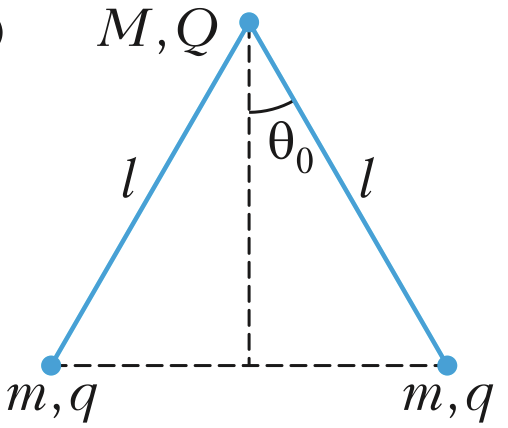
\includegraphics[width=.9\textwidth]{triangle.png}\\
        \begin{center}
            Рис.1 Начальная конфигурация
        \end{center}
    \end{minipage}
    \hfill
    \begin{minipage}{.38\textwidth}
        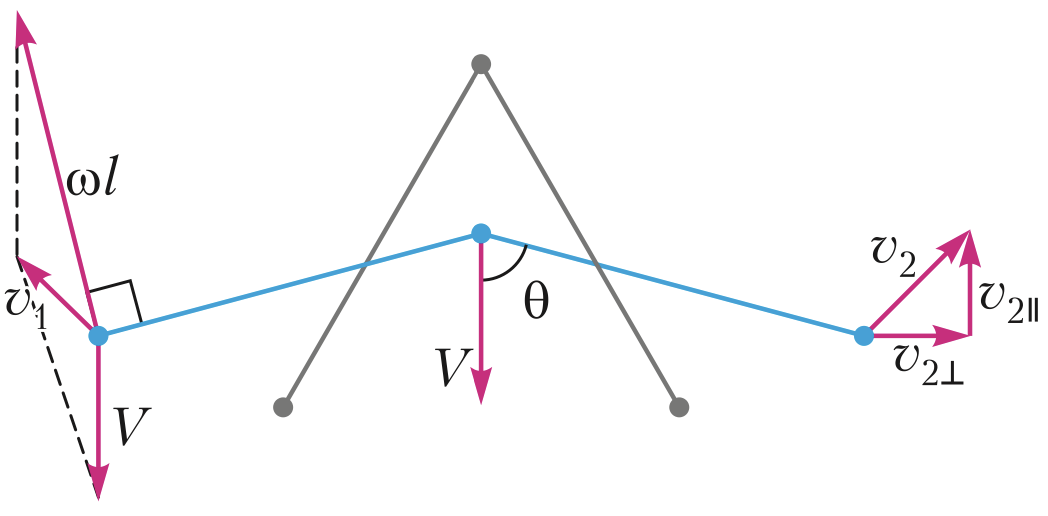
\includegraphics[width=.9\textwidth]{pronKonf.png}\\
        \begin{center}
            Рис.2 Промежуточная конфигурация
        \end{center}
    \end{minipage}
    \hfill
    \begin{minipage}{.35\textwidth}
        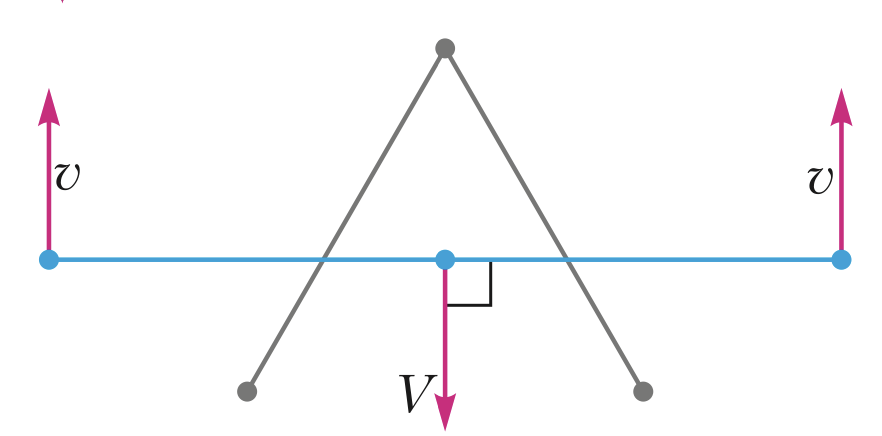
\includegraphics[width=.9\textwidth]{linealKonf.png}\\
        \begin{center}
            Рис.3 Линейная конфигурация
        \end{center}
    \end{minipage}
\end{center}
Вследствие симметрии действия электрических сил и сил натяжения нитей на центральный шарик он будет двигаться прямолинейно и ускоренно на всей первой четверти цикла вплоть до линейной конфигурации системы. В этом положении действующая на него результирующая сила обращается в ноль, а величина скорости достигает максимального значения.

Для анализа скоростей запишем законы сохранения импульса и энергиив промежуточной конфигурации:

\begin{equation}
    M\vec{V}+m\vec{v_1}+m\vec{v_2}=0;\ \frac{MV^2}{2}+mv^2=\frac{kq^2}{2l}(\frac{1}{sin\theta_0}-\frac{1}{sin\theta})
\end{equation}

В линейной конфигурации:

\begin{equation}
    M\vec{V}+2m\vec{v}=0;\ \frac{MV^2}{2}+mv^2=\frac{kq^2}{2l}(\frac{1}{sin\theta_0}-1)
\end{equation}


\begin{equation}
    V_{max}=V(\theta =\frac{\pi}{2}) = \sqrt{\frac{mkq^2}{M(M+2m)l}}\left(\frac{1}{sin\theta_0}-1\right)
\end{equation}

\begin{equation}
    v\left(\theta = \frac{\pi}{2}\right)=\frac{1}{2}\sqrt{\frac{Mkq^2}{m(M+2m)l}}\left(\frac{1}{sin\theta_0}-1\right)
\end{equation}
При $\gamma >> 1$ центральный шарик практически неподвижен и боковые шарики, двигаясь по круговым траекториям радиусом $l$, проходят линейную конфигурацию с максимальными скоростями.
В противоположном случае $\gamma << 1$ боковые шарики движутся практически прямолинейно.
\\
Связь скоростей центрального и бокового шариков:

\begin{equation}
    v^2= \frac{kq^2}{2ml}\left(\frac{1}{sin\theta_0}-\frac{1}{sin\theta}\right)\left(\frac{1-(1+2\gamma)(\frac{sin\theta}{1+\gamma})^2}{1-(1+\gamma)(\frac{sin\theta}{1+\gamma})^2}\right)
\end{equation}
Исследование экстремума скорости бокового шарика в линейной конфигурации:
\begin{equation}
    v^2\left(\frac{\pi}{2}+\delta\right)=\left(\frac{kq^2}{2ml}\frac{\gamma}{\gamma+1}\left(\frac{1-sin\theta_0}{sin\theta_0}\right)\right)\cdot\left(1-\left(\frac{sin\theta_0}{2\left(1-sin\theta_0\right)}-\frac{1+\gamma}{\gamma^2}\right)\delta^2\right)
\end{equation}
\begin{equation}
    v^2\left(\frac{\pi}{2}\right)=
    \begin{cases}
        v^2_{max},\ if\ \left(\frac{sin\theta_0}{2\left(1-sin\theta_0\right)}-\frac{1+\gamma}{\gamma^2}\right)>0\\
        v^2_{min},\ if\ \left(\frac{sin\theta_0}{2\left(1-sin\theta_0\right)}-\frac{1+\gamma}{\gamma^2}\right)<0
    \end{cases}
\end{equation}
Маскимальная скорость бокового шарика, которая достигается в первой четверти цикла при $\theta_0<\theta<\frac{\pi}{2}$ для случая при:
\begin{equation}
    \left(\frac{sin\theta_0}{2\left(1-sin\theta_0\right)}-\frac{1+\gamma}{\gamma^2}\right)<0;\ 
    z=\frac{1+\gamma}{sin\theta}\ =>\ v^2(z)=\frac{kq^2}{2ml(1+\gamma)}\left(\frac{1+\gamma}{sin\theta_0-z}\right)\left(\frac{z^2-(1+2\gamma)}{z^2-(1+\gamma)}\right),\ z\in \left(1+\gamma,\ \frac{1+\gamma}{sin\theta_0}\right)
\end{equation}
\section{Вывод}



\end{document}


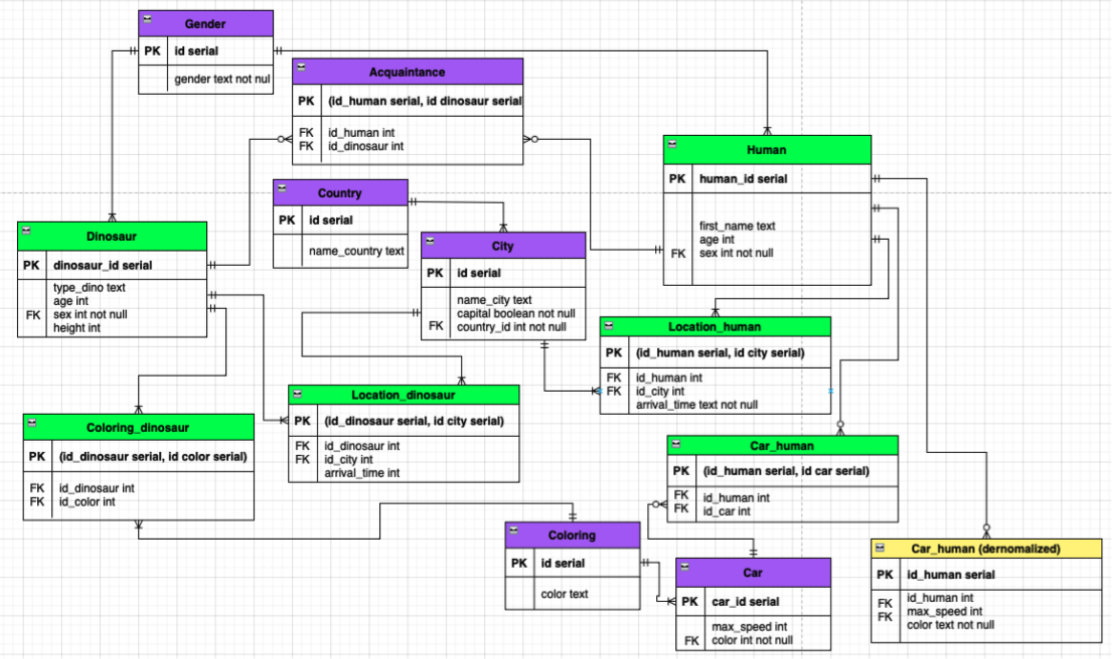
\includegraphics[width=.9\textwidth]{123}